%-- einleitung
\section{Konzept}
In diesem Abschnitt werden die konzeptionellen Planungen des Projekts mit Hilfe einer Anforderungsanalyse und einer Systemmodellierung dargstellt.

\subsection{Anforderungsanalyse}
In der Tabelle \ref{tab:fa} sind die funktionalen Anforderungen aufgelistet. Diese beschreiben, was in diesem Projekt alles Umgesetzt werden muss. Darunter sind eher triviale Punkte aber auch Vorgaben, wie zum Beispiel Daten eingelesen werden sollen.\\
In der Tabelle \ref{tab:nfa} sind die nichtfunktionalen Anforderungen aufgelistet. Diese hingegen beschreiben, wie das Projekt Umgesetzt werden soll. Hierunter Fallen Qualitätsvorgaben und Vorgaben über das Zielsystem.
Alle Anforderungen sind mit einer Nummer versehen, um im Laufe dieser Ausarbeitung leichter auf die Anforderungen verweisen zu können.

\begin{table}[H]
\caption{Funktionale Anforderungen}
\begin{tabular}{|c|p{12cm}|}
Nummer & Beschreibung \\
\hline
1FA & Die Liste der Städte (Namen + Distanzen) sollen aus einer Datei (mit bestimmter Formatierung) auslesbar sein, damit diese Daten ohne Programmieraufwand verändert werden können. \\  
2FA & Das System soll mit Genetischen Algorithmen das Travelling Salesman Problem umsetzen. \\  
3FA & Das System soll Routen auf Grundlage derer Gesamtdistanz beurteilen und weiterverarbeiten. \\  
\end{tabular}
\label{tab:fa}
\end{table}

\begin{table}[H]
\caption{Nichtfunktionale Anforderungen}
\begin{tabular}{|c|p{10cm}|}
 Nummer & Beschreibung \\ 
\hline
1NFA & Das System soll auf Windows 10 ausführbar sein.\\
2NFA & Das System soll vollständig dokumentiert sein.\\
3NFA & Das System soll leicht testbar sein.\\
4NFA & Das System soll leicht bedienbar sein.\\
5NFA & Das System soll als Executable ausführbar sein.\\
\end{tabular}
\label{tab:nfa}
\end{table}

\subsection{Systemmodellierung}

In Abbildung \ref{fig:systemmodellierung} ist ein FMC Diagramm zu sehen, das eine Übersicht über die Projektarchitektur bildet.
Die Genetischen Algorithmen werden innerhalb einer eigenen Library implementiert. Das hat den Vorteil, dass der Code somit eine hohe Wiederverwendbarkeit aufweist.
Innerhalb der Library verbirgt ein Simulator die Komplexität der eigentlichen Genetischen Algorithmen. Über den Simulator können Parametereinstellungen vorgenommen werden, die den Ablauf der Vorgänge steuern.
Der Simulator verwendet die Genetischen Algorithmen über einheitliche Schnittstellen, über die entweder Populationen oder Individuen ausgetauscht werden. Dadurch ist das System leicht bedienbar, was die Anforderung 4NFA erfüllt. Darüber hinaus ermöglicht diese klare Archtitektur eine leichte Testbarkeit und erüllt die Anforderung 3NFA. Die Library soll über ein Frontend ausgeführt werden und somit dem Benutzer die Möglichkeit geben einfach Simulationen durchzuführen. Dieses Projekt beschäftigt sich allerdings vornehmlich mit der Enwicklung der Library und weniger mit der Entwicklung des Frontends.

\begin{figure}[H]
\centering
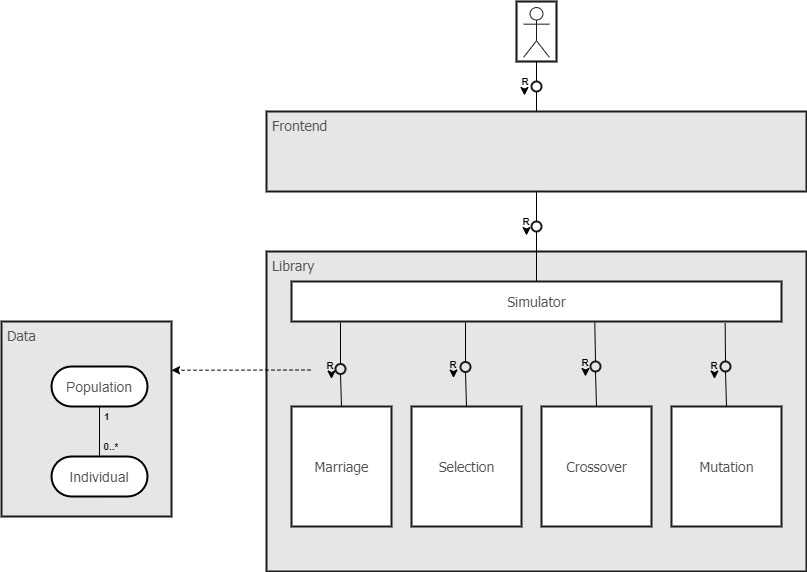
\includegraphics[width=1\textwidth]{img/Vortrag/Systemmodellierung.png}
\caption{Systemmodellierung}
\label{fig:systemmodellierung}
\end{figure}

%--